\documentclass{article}
\usepackage[landscape]{geometry}
\usepackage{url}
\usepackage{multicol}
\usepackage{amsmath}
\usepackage{esint}
\usepackage{amsfonts}
\usepackage{tikz}
\usetikzlibrary{decorations.pathmorphing}
\usepackage{amssymb}
\usepackage[version=4]{mhchem}
\usepackage{graphicx}
\usepackage{float}
\usepackage{colortbl}
\usepackage{xcolor}
\usepackage{mathtools}
\usepackage{enumitem}
\usepackage[symbol]{footmisc}
\makeatletter

\newcommand*\bigcdot{\mathpalette\bigcdot@{.5}}
\newcommand*\bigcdot@[2]{\mathbin{\vcenter{\hbox{\scalebox{#2}{$\m@th#1\bullet$}}}}}
\renewcommand{\thempfootnote}{\fnsymbol{mpfootnote}}
\makeatother

\title{Unit 3 - Thermochemistry and Chemical Kinetics}
\usepackage[T1]{fontenc}
\usepackage[utf8]{inputenc}
\usepackage[english]{babel}

\advance\topmargin-.8in
\advance\textheight3in
\advance\textwidth3in
\advance\oddsidemargin-1.5in
\advance\evensidemargin-1.5in
\parindent0pt
\parskip2pt
\newcommand{\hr}{\centerline{\rule{3.5in}{1pt}}}
%\colorbox[HTML]{e4e4e4}{\makebox[\textwidth-2\fboxsep][l]{texto}
\AtBeginEnvironment{align}{\setcounter{equation}{0}}
\begin{document}

\begin{center}{\huge{\textbf{Unit 3 - Thermochemistry}}}\\
\end{center}
\begin{multicols*}{3}

\tikzstyle{mybox} = [draw=black, fill=white, very thick,
    rectangle, rounded corners, inner sep=10pt, inner ysep=10pt]
\tikzstyle{fancytitle} =[fill=black, text=white, font=\bfseries]

%------------ Thermochemistry ---------------
\begin{tikzpicture}
\node [mybox] (box){%
    \begin{minipage}{0.3\textwidth}
    \textbf{Thermochemistry}: the study of the energy changes involved in chemical and physical processes.
    \begin{itemize}
        \item kinetic energy is the energy of motion
	\item potential energy is the stored energy an object has as a result of its condition
	\item the joule (J) is equivalent to a kg$\cdot$m$^{2}$/s$^{2}$
	\item 1 kJ = 1000 J
	\item the density of water is 1.00 g/mL
	\item $\Delta T$ = $T$\textsubscript{final} $-$ $T$\textsubscript{initial}
    \end{itemize}
    \textbf{Thermal Energy}: the sum of all the kinetic energies of all the particles of a sample of matter. \\
    \textbf{Temperature}: a measure of the average kinetic energy of all the particles of a sample of matter. \\
    The $\Delta T$ is dependent on:
    \begin{itemize}
        \item amount of heat exchanged
        \item mass of the substance being measured
	\item type of substance being measured
    \end{itemize}
    \textbf{Endothermic}: describes the process during which heat enters a system. \\
    $\hookrightarrow$ $\Delta H$ is $+$ve because the enthalpy of the system $\uparrow$ \\
    \textbf{Exothermic}: describes the process during which heat leaves a system. \\
    $\hookrightarrow$ $\Delta H$ is $-$ve because the enthalpy of the system $\downarrow$ \\
    A \textit{system} is the object or substance being studied, and the \textit{surroundings} are everything else in the universe. \\
    \textbf{Open System}: a system that can exchange both matter and energy with the surroundings. \\
    e.g. uncovered pot of potatoes boiling on the stove \\
    \textbf{Closed System}: a system that can exchange only energy with the surroundings. \\
    e.g. pressure cooker with potatoes boiling on the stove \\
    \textbf{Isolated System}: a system that cannot exchange either energy or matter with the surroundings. \\
    e.g. a pot of potatoes inside an insulated container \\
    $\star$ It is difficult to completely isolate a system; there is no truly isolated system except the universe itself.
    \end{minipage}
};
%------------ Thermochemistry Header ---------------------
\node[fancytitle, right=10pt] at (box.north west) {Thermochemistry};
\end{tikzpicture}

%------------ First Law of Thermodynamics ---------------
\begin{tikzpicture}
\node [mybox] (box){%
    \begin{minipage}{0.3\textwidth}
    \textbf{First Law of Thermodynamics}: energy can be converted from one form to another but cannot be created or destroyed.
    \begin{itemize}
        \item $E$\textsubscript{universe} = constant
	\item $\Delta E$\textsubscript{universe} = 0
	\item universe = system + surroundings
	\item $E$\textsubscript{universe} = $E$\textsubscript{system} + $E$\textsubscript{surroundings}
	\item $\Delta E$\textsubscript{universe} = $\Delta E$\textsubscript{system} + $\Delta E$\textsubscript{surroundings} = 0
	\item $\Delta E$\textsubscript{system} = $-\Delta E$\textsubscript{surroundings}
    \end{itemize}
    When a system absorbs energy, the surroundings release it and when a system releases energy, the surroundings absorb it.
    \end{minipage}
};
%------------ First Law of Thermodynamics Header ---------------------
\node[fancytitle, right=10pt] at (box.north west) {First Law of Thermodynamics};
\end{tikzpicture}

%------------ Enthalpy ---------------
\begin{tikzpicture}
\node [mybox] (box){%
    \begin{minipage}{0.3\textwidth}
    \textbf{Enthalpy, \textit{H}}: the total energy of the system plus the pressure times the volume, or $H=E+PV$. \\
    e.g. \ce{CO(g) + 2H2(g) -> CH3OH(l) + 128.6 kJ} or \\
    \ce{CO(g) + 2H2(g) -> CH3OH(l)} $\Delta H=-128.6\text{ kJ}$ \\
    $\rightarrow$ Sometimes called the \textit{heat content} of the system. \\
    $\rightarrow$ The enthalpy change of a system depends only on the initial state (condition) and on the final state of the system and is represented as $\Delta H=\Delta E+\Delta(PV)$. \\
    \textbf{Enthalpy of Solution, $\Delta H$\textsubscript{solution}}: the enthalpy change associated with a solute dissolving in a solvent.
    \begin{itemize}
        \item bond energy is the energy required to break a chemical bond
	\item larger bond energies result in stabler bonds
	\item stable bonds have low potential energy
    \end{itemize}
    $\Delta H=\text{Reactant Bond energy}-\text{Product Bond energy}$ \\
    $\rightarrow$ The difference between the total amount of energy used to break bonds and the total energy released when the bonds reform is equal to the enthalpy change of the reaction. \\
    $\star$ Strong bonds have low potential energy and weak bonds have high potential energy.
    \end{minipage}
};
%------------ Enthalpy Header ---------------------
\node[fancytitle, right=10pt] at (box.north west) {Enthalpy};
\end{tikzpicture}

%------------ Second Law of Thermodynamics ---------------
\begin{tikzpicture}
\node [mybox] (box){%
    \begin{minipage}{0.3\textwidth}
    \textbf{Second Law of Thermodynamics}: when two objects are in thermal contact, heat is always transferred from the object at a higher temperature to the object at a lower temperature until the two objects are at the same temperature (related to entropy). \\
    $\star$ When two systems have reached the same temperature, they are in \textit{thermal equilibrium}.
    \end{minipage}
};
%------------ Second Law of Thermodynamics Header ---------------------
\node[fancytitle, right=10pt] at (box.north west) {Second Law of Thermodynamics};
\end{tikzpicture}

%------------ Calorimetry ---------------
\begin{tikzpicture}
\node [mybox] (box){%
    \begin{minipage}{0.3\textwidth}
    The following equation enables you to calculate the amount of heat absorbed or released by a substance. \\
    e.g. the \textit{law of conservation of energy} \\ \\
    $\boxed{Q=m\cdot c\cdot\Delta T}$
    \begin{itemize}
        \item Q $\rightarrow$ heat (J)
	\item m $\rightarrow$ mass (g)
	\item c $\rightarrow$ specific heat capacity ($\text{J/g}\cdot^{\circ}\text{C}$)
	\item $\Delta T$ $\rightarrow$ change in temperature ($^{\circ}$C)
    \end{itemize}
    $\rightarrow$ If $\Delta T$ is positive, then $Q$ is positive. \\
    $+$ve value for $Q$ means that heat entered the system. \\
    $\rightarrow$ If $\Delta T$ is negative, then $Q$ is negative. \\
    $-$ve value for $Q$ means that heat left the system. \\
    \textbf{Specific Heat Capacity, \textit{c}}: the amount of energy needed to increase the temperature of one gram of a substance by one degree Celsius. \\
    Q: If the same amount of heat were added to 1 g samples of water, methanol, and aluminum, which substance would undergo the greatest $\Delta T$?
    \begin{itemize}
        \item $c$\textsubscript{water} = 4.19 $\text{J/g}\cdot^{\circ}\text{C}$
        \item $c$\textsubscript{methanol} = 2.918 $\text{J/g}\cdot^{\circ}\text{C}$
        \item $c$\textsubscript{aluminum} = 0.900 $\text{J/g}\cdot^{\circ}\text{C}$
    \end{itemize}
    A: Aluminum would undergo the greatest temperature change because it requires the least amount of energy to increase the temperature of one gram of it. \\
    $\star$ The range of enthalpy changes is lowest for physical changes, intermediate for chemical changes, and highest for nuclear changes.
    \end{minipage}
};
%------------ Calorimetry Header ---------------------
\node[fancytitle, right=10pt] at (box.north west) {Calorimetry};
\end{tikzpicture}

%------------ Molar Enthalpy of Combustion ---------------
\begin{tikzpicture}
\node [mybox] (box){%
    \begin{minipage}{0.3\textwidth}
    \textbf{Standard Enthalpy of a Reaction, $\Delta H_{\text{r}}^\circ$}: the enthalpy change for the amount in moles of each reactant and product as determined by the coefficient of the term in the chemical equation. \\
    $\rightarrow$ The enthalpy change of a reaction is equal to the amount in moles, $n$, of a specified reactant or product multiplied by the standard molar enthalpy change for the specified reactant or product. \\ \\
    $\boxed{\Delta H_{\text{r}}=n\Delta H_{\text{r}}^\circ}$ or $\boxed{\Delta H_{\text{comb}}=n\Delta H_{\text{comb}}^\circ}$
    \begin{itemize}
        \item $\Delta H_{\text{comb}}$ represents enthalpy of combustion
        \item $\Delta H_{\text{comb}}^\circ$ represents the standard molar enthalpy of combustion
    \end{itemize}
    $\rightarrow$ If you know the enthalpy of a reaction, you can use it to determine the amounts of the reactants or products involved. \\
    $\star$ It is not possible to measure the total enthalpy of a system, but it is possible to measure the \textit{change} in the enthalpy of a system.
    \end{minipage}
};
%------------ Molar Enthalpy of Combustion Header ---------------------
\node[fancytitle, right=10pt] at (box.north west) {Molar Enthalpy of Combustion};
\end{tikzpicture}

%------------ Calorimeter ---------------
\begin{tikzpicture}
\node [mybox] (box){%
    \begin{minipage}{0.3\textwidth}
    \textbf{Calorimeter}: a device used to measure the heat released or absorbed during a chemical or physical process occurring within it. \\
    \textbf{Simple Calorimeter}: a calorimeter made of two stacked vessels covered by a lid with holes in the top just large enough for a thermometer and a stirrer.
    \begin{itemize}
	\item the process takes place under constant pressure
	\item the amount of heat that is exchanged between the calorimeter and the system is equal to the change in the enthalpy of the system
    \end{itemize}
    \textbf{Bomb Calorimeter}: measures heat released during a combustion reaction at a constant volume.
    \begin{itemize}
        \item the reaction takes place inside an inner metal chamber, called a \textit{bomb}
	\item the reactants are ignited using an electrical coil
	\item the units of $C$ are joules per degree Celsius
    \end{itemize}
    $C_{\text{bomb calorimeter}}=C_{\text{water}}+C_{\text{thermometer}}+C_{\text{stirrer}}+C_{\text{container}}$
    \end{minipage}
};
%------------ Molar Enthalpy Header ---------------------
\node[fancytitle, right=10pt] at (box.north west) {Calorimeter};
\end{tikzpicture}

%------------ Thermochemical Equations ---------------
\begin{tikzpicture}
\node [mybox] (box){%
    \begin{minipage}{0.3\textwidth}
    The enthalpy of a reaction is directly proportional to the amounts of the substances that react. \\
    What is the thermochemical equation for this dissolution? Given: \\
    $m\textsubscript{NaOH}$ = 5.50 g, $V\textsubscript{water}$ = 175 mL, $\Delta T\textsubscript{water}=2.1^{\circ}\text{C}$
    \begin{align}
    q\textsubscript{water}&=m\textsubscript{water}+c\textsubscript{water}+\Delta T_\textsubscript{water} \\
    &=(175\text{ g})(4.184\text{ J/g$^{\circ}$C})(2.1^{\circ}\text{C}) \\
    &=1537.62\text{ J}\text{ or }1.53762\text{ kJ}
    \end{align}
    $\displaystyle{n\textsubscript{NaOH}=\frac{5.50\text{ g}}{39.9971\text{ g/mol}}\approx0.13751\text{ mol}}$ \\ \\
    $\displaystyle{\Delta H_{\text{rxn}}^\circ=\frac{-1.53762\text{ kJ}}{0.13751\text{ mol}}\approx-11\text{ kJ/mol}}$ \\ \\
    \ce{NaOH(s) -> NaOH(aq) + 11 kJ} \\
    $\star$ Divide the enthalpy of the reaction by the moles of the reactant to solve for the enthalpy term.
    \end{minipage}
};
%------------ Thermochemical Equations Header ---------------------
\node[fancytitle, right=10pt] at (box.north west) {Thermochemical Equations};
\end{tikzpicture}

%------------ Potential Energy Diagram ---------------
\begin{tikzpicture}
\node [mybox] (box){%
    \begin{minipage}{0.3\textwidth}
    The slow step (rate-determining) in a chemical process is the step with the highest activation energy.
    \begin{itemize}
        \item breaking a bond is an endothermic process
        \item forming a bond is an exothermic process
    \end{itemize}
    \begin{figure}[H]
        \centering
        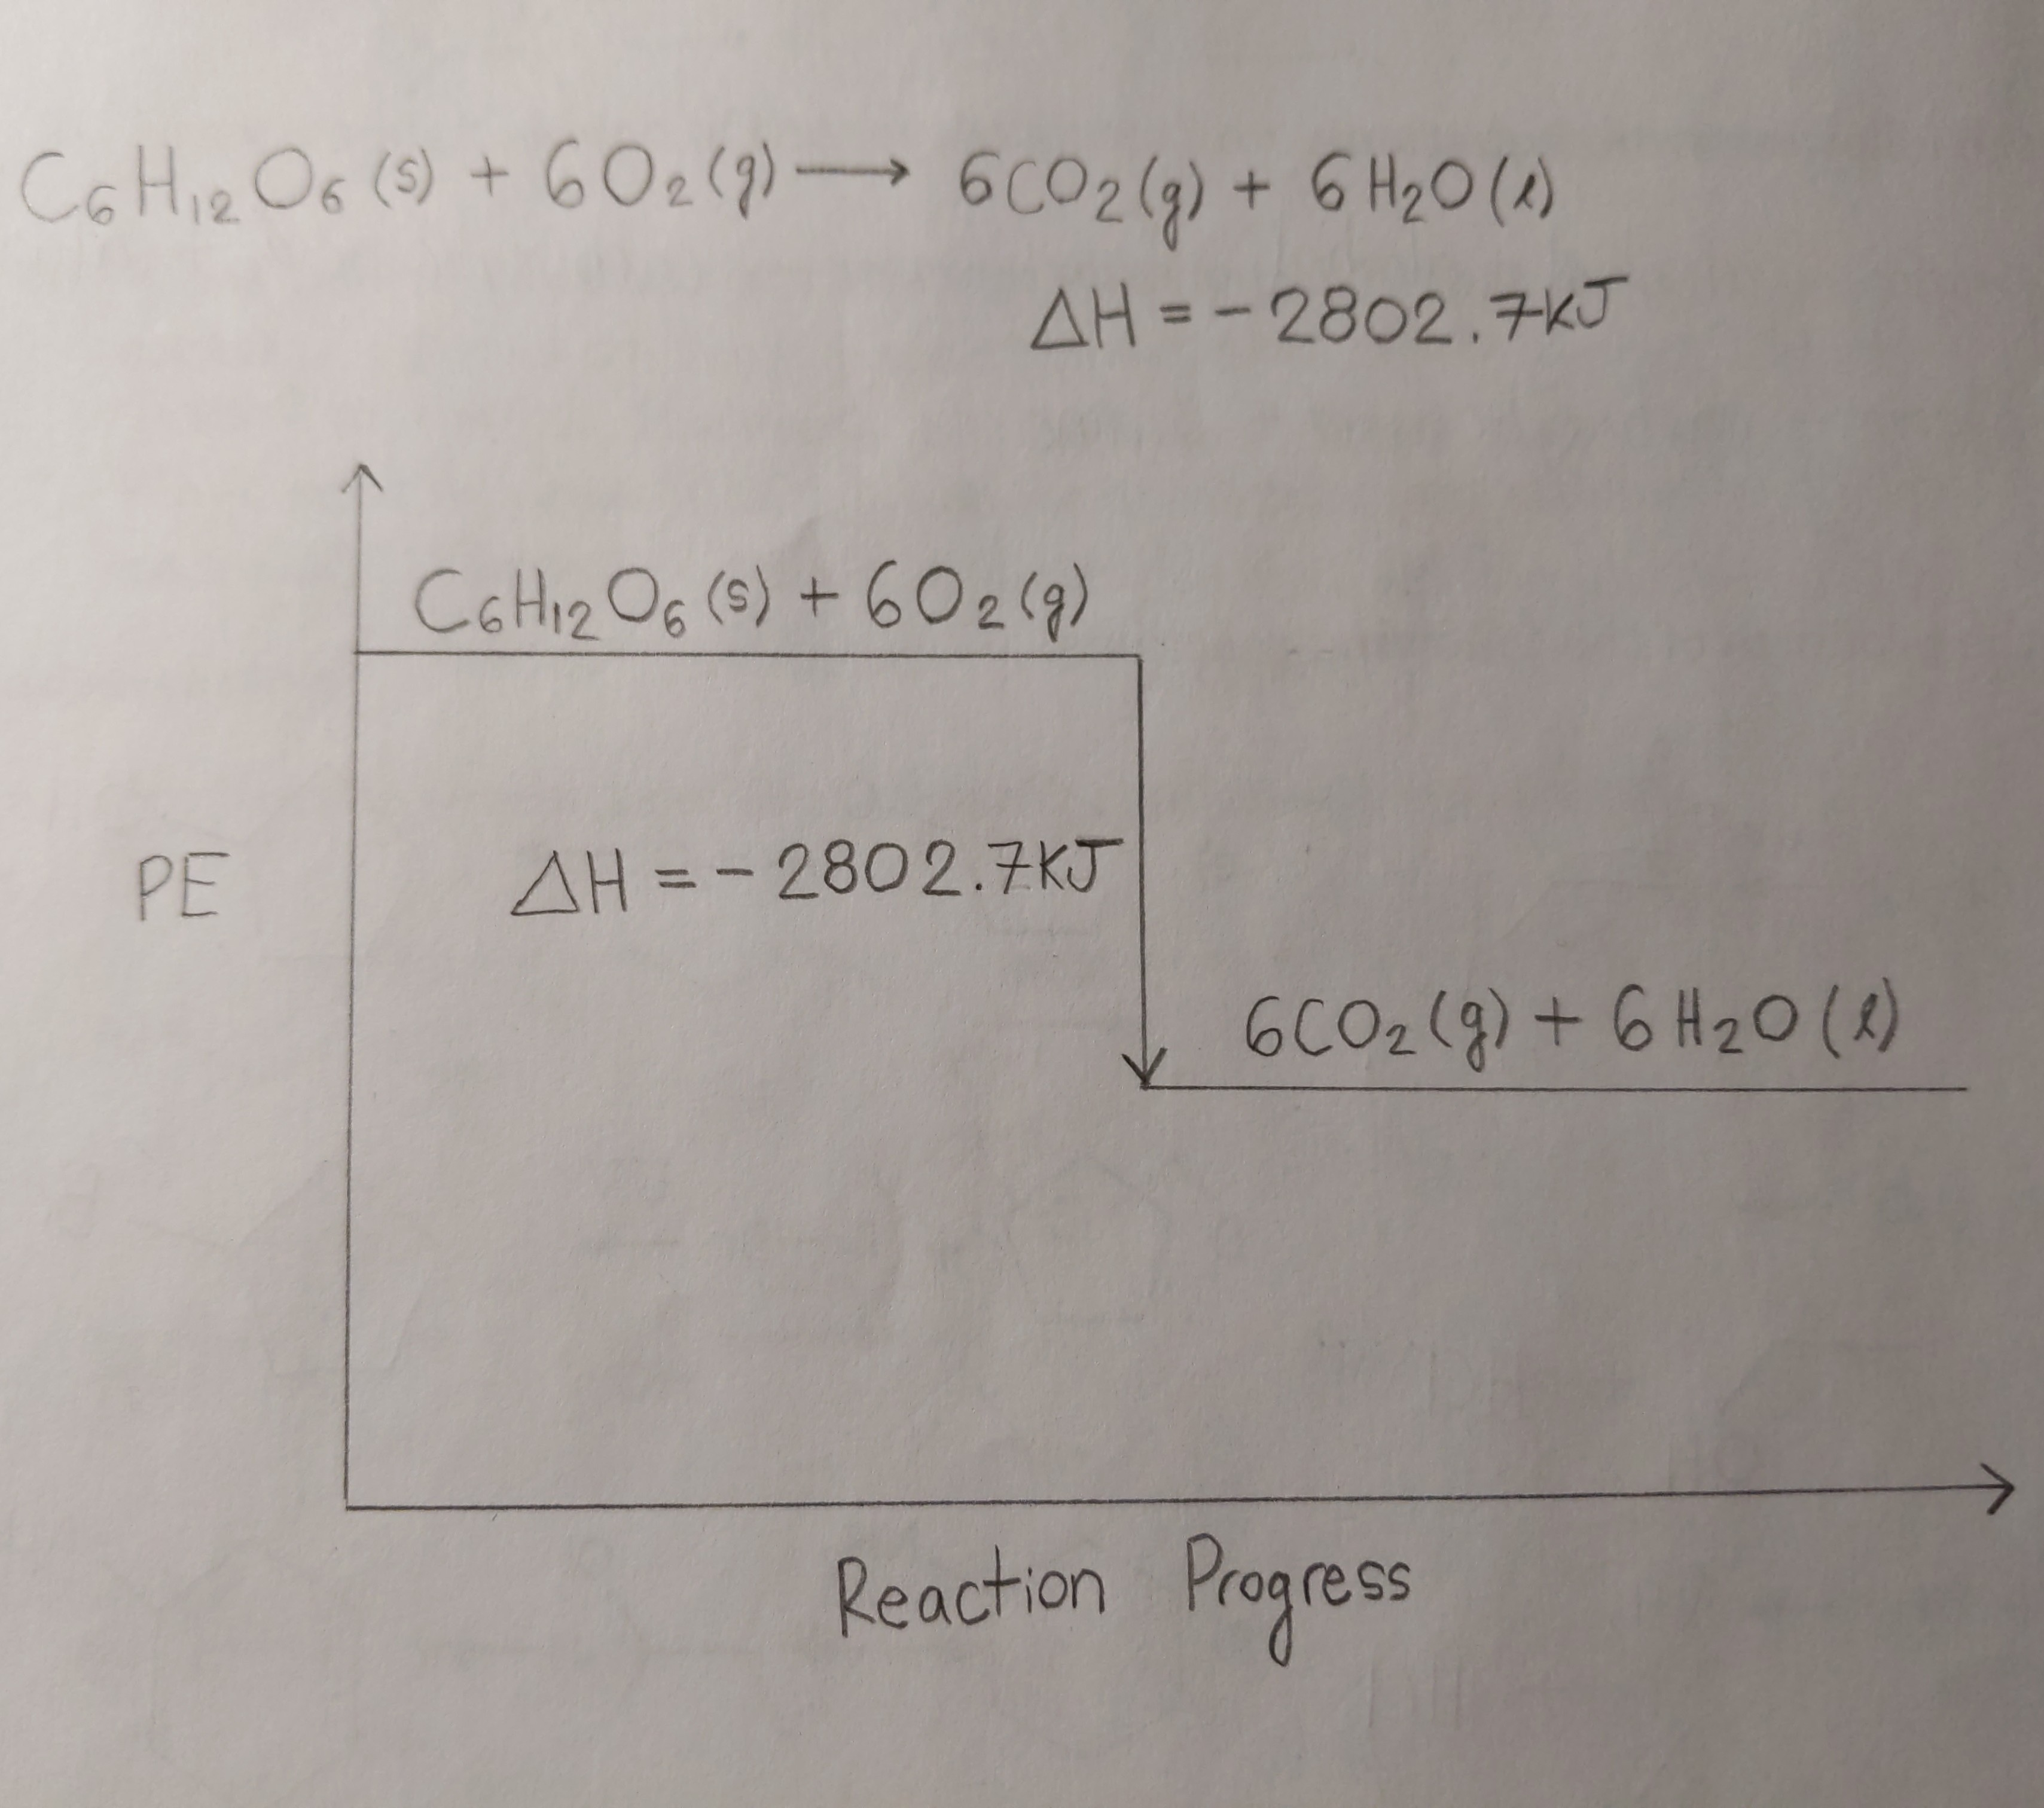
\includegraphics[scale=0.062]{diagrams/potential-energy.jpg}
        \label{fig:potential}
    \end{figure}
    $\star$ There is no difference in enthalpy change for the catalyzed and the uncatalyzed reaction.
    \end{minipage}
};
%------------ Potential Energy Diagram Header ---------------------
\node[fancytitle, right=10pt] at (box.north west) {Potential Energy Diagram};
\end{tikzpicture}

%------------ Hess's Law ---------------
\begin{tikzpicture}
\node [mybox] (box){%
    \begin{minipage}{0.3\textwidth}
    \textbf{Hess's Law}: the enthalpy change of a physical or chemical process depends only on the initial and final conditions of the process. The enthalpy change of a multistep process is the sum of the enthalpy changes of its individual steps. \\
    \textbf{Manipulating chemical equations}:
    \begin{figure}[H]
        \centering
        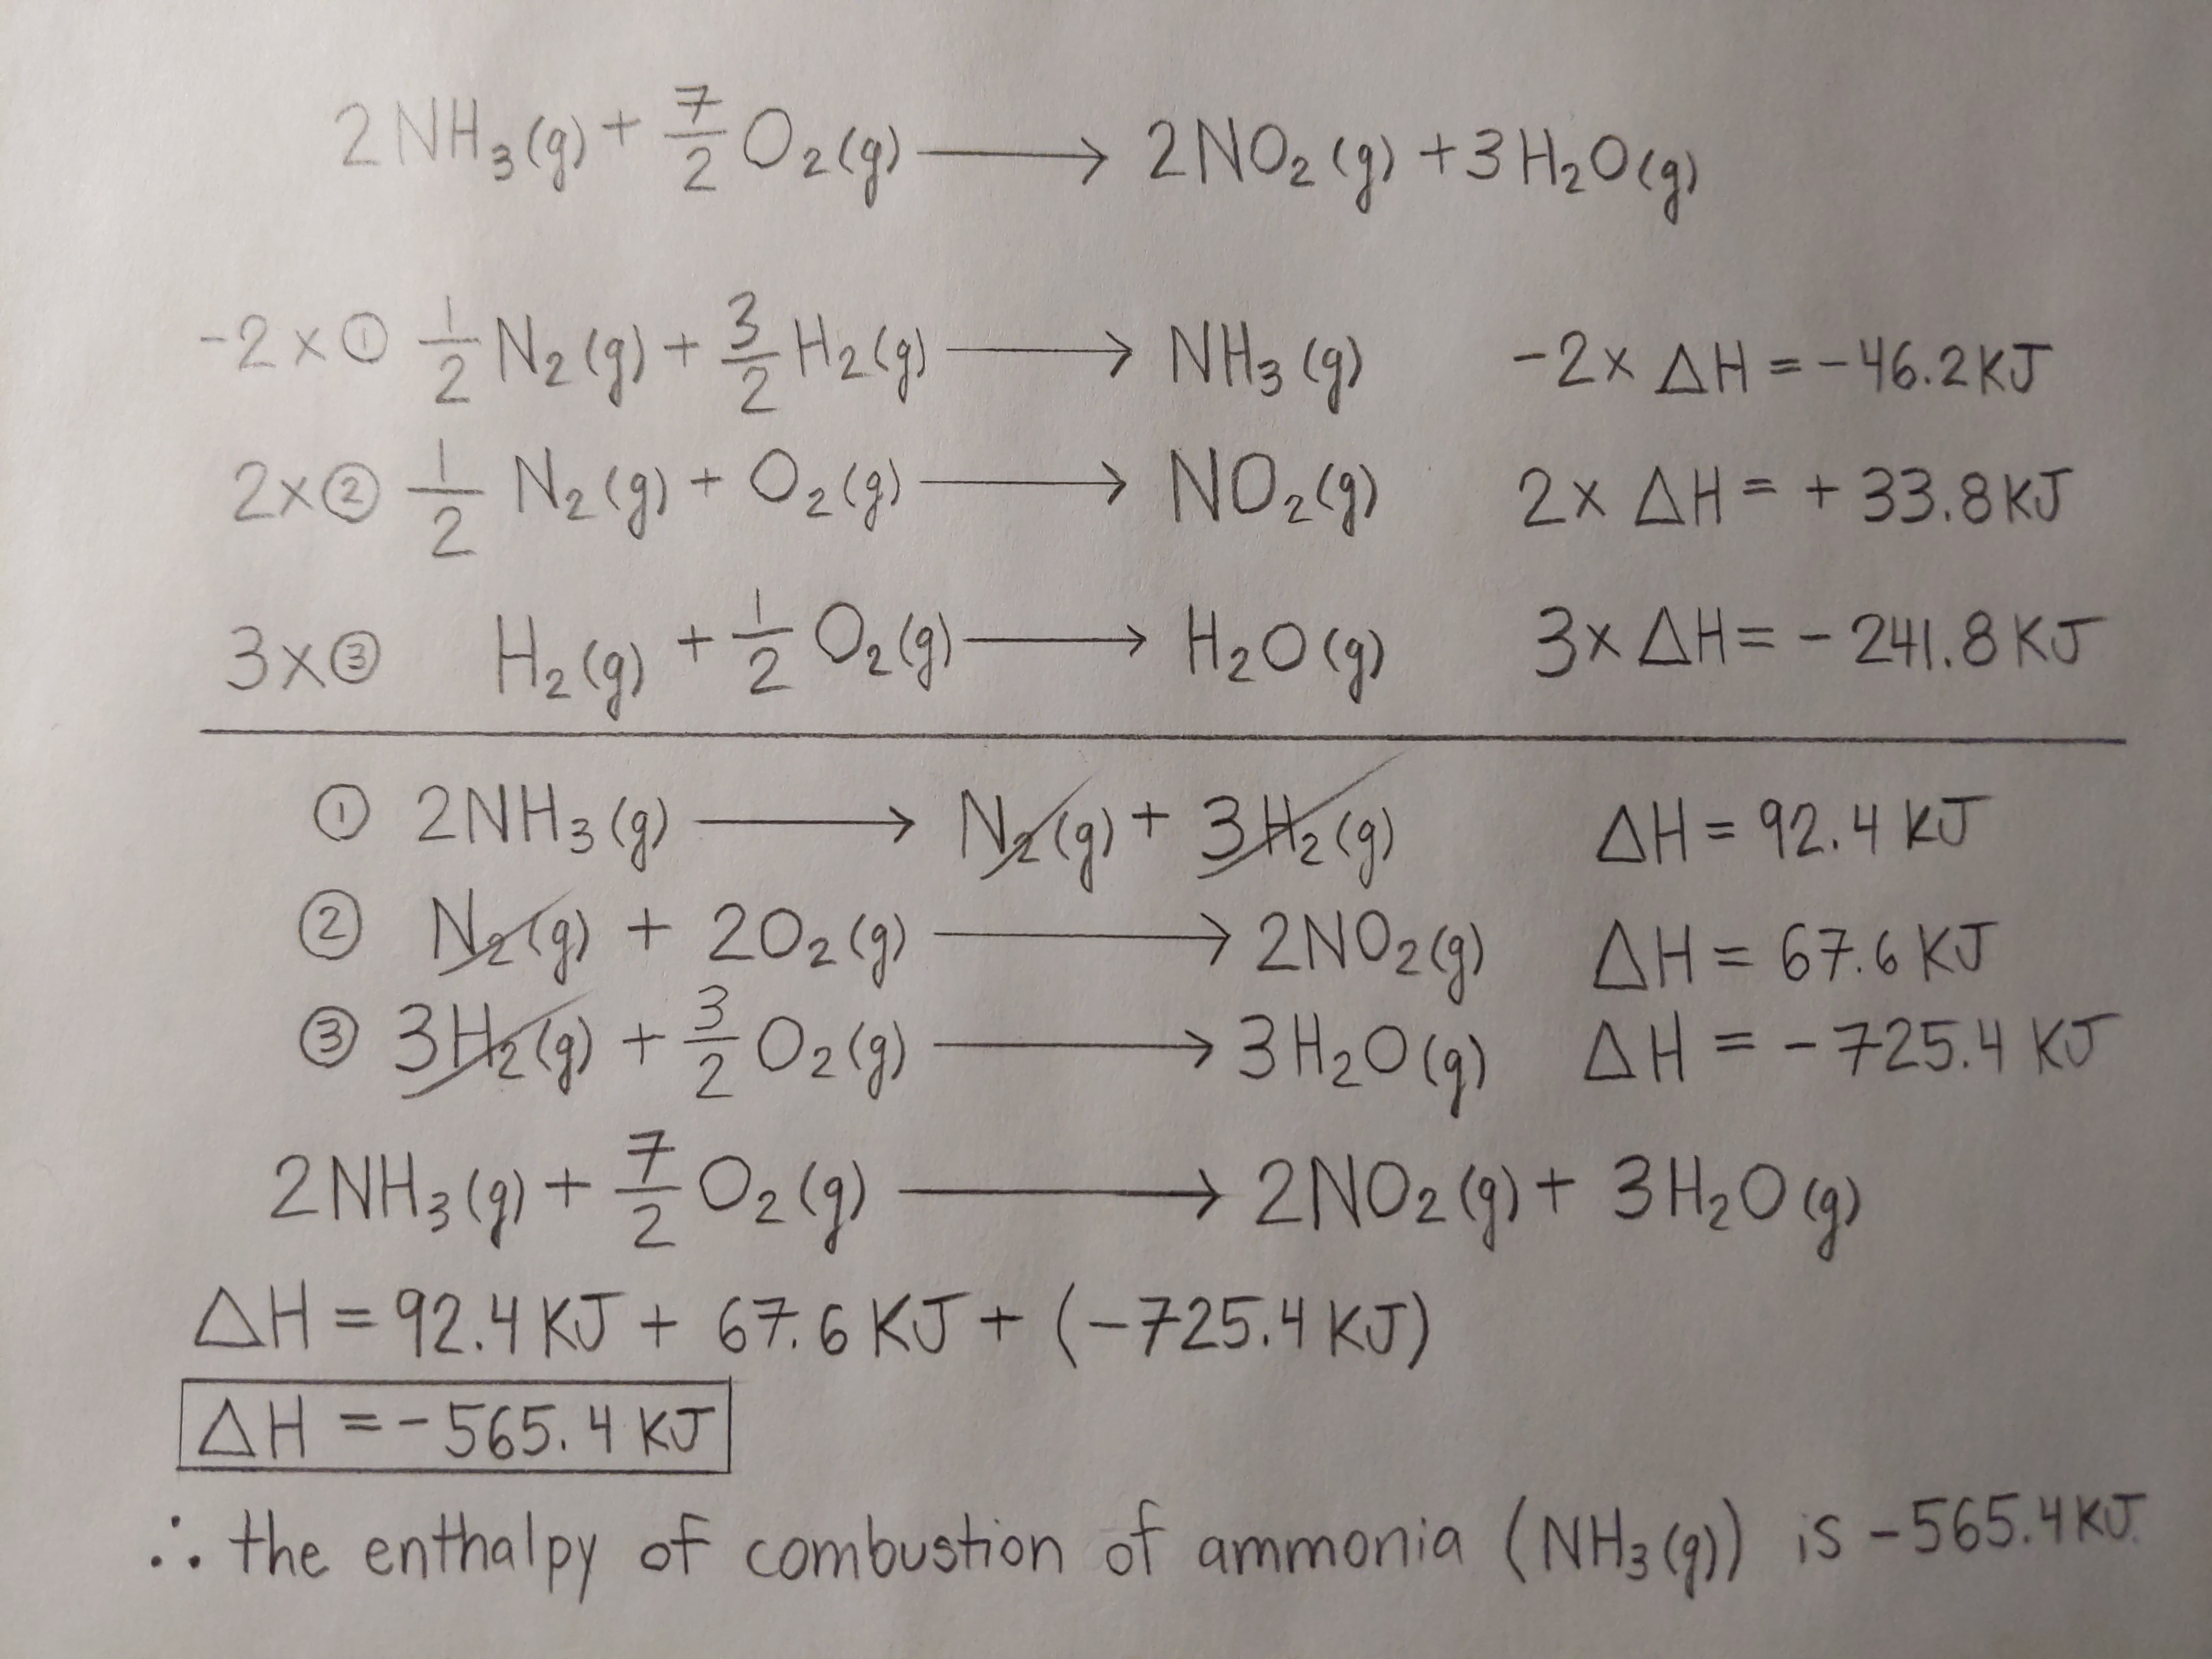
\includegraphics[scale=0.056]{diagrams/hess-law.jpg}
        \label{fig:hess}
    \end{figure}
    \begin{itemize}
        \item if you multiply by a constant, you must multiply the enthalpy change by that same constant
	\item if you reverse an equation, you must change the sign of the enthalpy change
    \end{itemize}
    \textbf{Standard Molar Enthalpy of Formation, $\Delta H_{\text{f}}^\circ$}: the change in enthalpy when 1 mol of a compound is formed directly from its elements in their most stable state at SATP (25$^{\circ}$C and 100 kPa). \\
    $\boxed{\Delta H_{\text{r}}^\circ=\sum(n\Delta H_{\text{f}}^\circ\text{products})-\sum(n\Delta H_{\text{f}}^\circ\text{reactants})}$
    \begin{itemize}
	\item $\Delta H_{\text{r}}^\circ$ represents the enthalpy change of a chemical reaction
        \item $n$ represents the stoichiometric coefficients for each substance
	\item $\sum$ means ``the sum of''
    \end{itemize}
    \textbf{Note}: Oxygen gas, \ce{O2(g)}, at SATP is an element in its most stable state. Therefore, its standard enthalpy of formation is zero. \\
    $\star$ The reactants do not actually break down into their elements and then react to form products.
    \end{minipage}
};
%------------ Hess's Law Header ---------------------
\node[fancytitle, right=10pt] at (box.north west) {Hess's Law};
\end{tikzpicture}

\end{multicols*}

\begin{center}{\huge{\textbf{Unit 3 - Chemical Kinetics}}}\\
\end{center}
\begin{multicols*}{3}

\tikzstyle{mybox} = [draw=black, fill=white, very thick,
    rectangle, rounded corners, inner sep=10pt, inner ysep=10pt]
\tikzstyle{fancytitle} =[fill=black, text=white, font=\bfseries]

%------------ Reaction Rates ---------------
\begin{tikzpicture}
\node [mybox] (box){%
    \begin{minipage}{0.3\textwidth}
    \textbf{Reaction Rate}: the speed at which a reaction occurs, or the change in the amount of reactants consumed or products formed over a given time interval.
    \begin{align}
    \text{reaction rate}&=\frac{\text{[A]}\textsubscript{final}-\text{[A]}\textsubscript{initial}}{t\textsubscript{final}-t\textsubscript{initial}} \\
    &=\frac{\Delta \text{[A]}}{\Delta t}
    \end{align}
    $\rightarrow$ The square brackets represent concentration. \\
    \textbf{Rate Law}: a mathematical relationship that must be experimentally determined for a chemical reaction. \\
    $\text{rate}=k\text{[A]}^m\text{[B]}^n$, where $k$ is the \textit{rate constant}. \\
    $\rightarrow$ The order of the overall reaction is $m+n$. \\
    \textbf{Average Rate of Reaction}: the change in the concentration of a reactant or product per unit time over a given time interval as a chemical reaction proceeds. \\
    $\rightarrow$ Calculate the slope of a line drawn between the two points that define the time interval. \\
    \textbf{Instantaneous Rate of Reaction}: the rate of a chemical reaction at a particular point in time. \\
    $\rightarrow$ Can be found by calculating the slope of a line that is tangent to that particular point in time. \\
    Factors that affect the rate of reaction:
    \begin{itemize}
        \item $\uparrow$ temperature = $\uparrow$ kinetic energy
	\item $\uparrow$ concentration of reactants = $\uparrow$ collisions
	\item catalysts = lowers the activation energy
	\item $\uparrow$ surface area of a solid reactant = $\uparrow$ \# of sites
	\item $\uparrow$ pressure of gaseous reactants and products = $\uparrow$ collisions due to molecules being closer together
    \end{itemize}
    $\star$ A reaction rate is always expressed as a $+$ve value.
    \end{minipage}
};
%------------ Reaction Rates Header ---------------------
\node[fancytitle, right=10pt] at (box.north west) {Reaction Rates};
\end{tikzpicture}

%------------ Activation Energy ---------------
\begin{tikzpicture}
\node [mybox] (box){%
    \begin{minipage}{0.3\textwidth}
    \textbf{Activation Energy, $E\textsubscript{a}$}: the minimum amount of energy (collision energy) required to initiate a chemical reaction. \\
    For an exothermic reaction: $E\textsubscript{a(rev)}=E\textsubscript{a(fwd)}+\Delta H$ \\
    For an endothermic reaction: $E\textsubscript{a(rev)}=E\textsubscript{a(fwd)}-\Delta H$ \\
    $\star$ The activation energy is independent of temperature; it does not change when temperature changes.
    \end{minipage}
};
%------------ Activation Energy Header ---------------------
\node[fancytitle, right=10pt] at (box.north west) {Activation Energy};
\end{tikzpicture}

%------------ Entropy and Spontaneity ---------------
\begin{tikzpicture}
\node [mybox] (box){%
    \begin{minipage}{0.3\textwidth}
    \textbf{Spontaneous}: processes that occur on their own in one particular direction. \\
    $\rightarrow$ Enthalpy is not the main determining factor in spontaneity (common misconception). \\
    \textbf{Entropy, \textit{S}}: the degree of molecular randomness or disorder in a system. \\
    $\rightarrow$ An increase in entropy is the main contributing factor in determining spontaneity. \\
    $\hookrightarrow$ Processes tend towards the higher entropy state due to probabilities. \\
    $\hookrightarrow$ The most probable state is the most likely to be observed. \\ \\
    $\displaystyle{p=\frac{\text{\# microstates that create an arrangement}}{\text{total \# microstates possible}}}$ \\
    \begin{itemize}
        \item the largest \# of microstates is the most likely to be observed (even distribution of atoms)
	\item such an arrangement has the highest entropy
    \end{itemize}
    \textbf{Second Law of Thermodynamics}: the universe tends towards increasing entropy, $\Delta S\textsubscript{universe}\geq0$. \\
    $\rightarrow$ Systems tend to go toward higher entropy states.
    Entropy changes involved with state changes:
    \begin{itemize}
        \item solid < liquid < gas, a substance changes state from a more ordered state to a less ordered state
	\item there are fewer microstates available in solids due to the restriction of motion
	\item more microstates are allowed for substances in the liquid or gaseous state
    \end{itemize}
    $\Delta S > 0$ if
    \begin{itemize}
        \item there are more moles of the products than reactants
        \item complex molecules are broken into smaller molecules
    \end{itemize}
    Q: Which of the following has a higher entropy? 1 mol of \ce{H2O(s)} or \ce{H2O(g)} at a given temp.? 1 mol of \ce{H2(g)} at 1 atm or 0.01 atm at a given temp.? \\
    A: \ce{H2O(g)} > \ce{H2O(s)} and 0.01 atm > 1 atm
    \end{minipage}
};
%------------ Entropy and Spontaneity Header ---------------------
\node[fancytitle, right=10pt] at (box.north west) {Entropy and Spontaneity};
\end{tikzpicture}

%------------ Gibbs Free Energy ---------------
\begin{tikzpicture}
\node [mybox] (box){%
    \begin{minipage}{0.3\textwidth}
    \textbf{Gibbs Free Energy, \textit{G}}: the amount of energy available to do work in a chemical system. \\
    $\boxed{\Delta G=\Delta H-T\Delta S}$ \\ \\
    $\boxed{\Delta S^\circ=\sum(n\Delta S^\circ\text{products})-\sum(n\Delta S^\circ\text{reactants})}$ \\ \\
    Exergonic reactions
    \begin{itemize}
	\item release energy $\rightarrow$ spontaneous
	\item $\Delta G<0$
    \end{itemize}
    Endergonic reactions
    \begin{itemize}
	\item absorb energy $\rightarrow$ non-spontaneous
	\item $\Delta G>0$
    \end{itemize}
    \end{minipage}
};
%------------ Gibbs Free Energy Header ---------------------
\node[fancytitle, right=10pt] at (box.north west) {Gibbs Free Energy};
\end{tikzpicture}

%------------ Collision Theory ---------------
\begin{tikzpicture}
\node [mybox] (box){%
    \begin{minipage}{0.3\textwidth}
    \textbf{Collision Theory}: the theory that a reaction occurs between two particles (atoms, molecules, or ions) if they collide at the correct orientation and with a certain minimum energy. \\
    For a collision between reactants to be effective:
    \begin{enumerate}
        \item the orientation of the reactants (the collision geometry) must be favourable.
	\item the collision must occur with sufficient energy.
    \end{enumerate}
    The area under a \textit{Maxwell-Boltzmann distribution} curve represents the distribution of the kinetic energy of collisions at a given temperature.
    \end{minipage}
};
%------------ Collision Theory Header ---------------------
\node[fancytitle, right=10pt] at (box.north west) {Collision Theory};
\end{tikzpicture}

%------------ Activated Complex ---------------
\begin{tikzpicture}
\node [mybox] (box){%
    \begin{minipage}{0.3\textwidth}
    \textbf{Activated Complex}: a chemical species temporarily formed by the colliding reactant molecules before the final product of the reaction is formed. \\
    $\rightarrow$ It is a temporary arrangement of atoms that form as bonds are breaking and new bonds are forming. \\
    \textbf{Transition State}: point when reactant(s) are converted to product(s). \\
    $\star$ Activated complex refers to all possible intermediates whereas the transition state refers to the intermediate with the highest potential energy.
    \end{minipage}
};
%------------ Activated Complex Header ---------------------
\node[fancytitle, right=10pt] at (box.north west) {Activated Complex};
\end{tikzpicture}

\end{multicols*}
\end{document}
